\documentclass{standalone}
\usepackage{tikz}
\usetikzlibrary{decorations.pathreplacing}
\usepackage{amsfonts}


\begin{document}
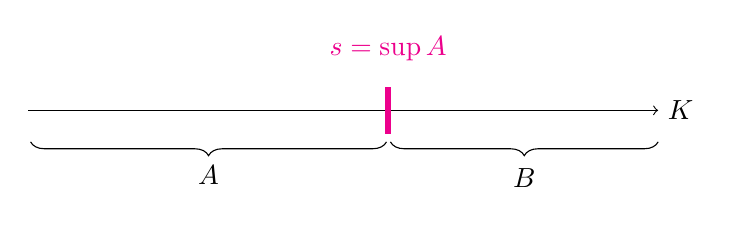
\begin{tikzpicture}
% Draw the real line
  \draw[->] (-4,0) -- (4,0) node[right] {$K$};
  
  % Draw the point 'x' and '0'

 


  

  
  % Draw the brace and label it
  \draw[decorate,decoration={brace,mirror,amplitude=5pt}] (-3.97,-0.4) -- (0.55,-0.4) node[midway,below=5pt] {$A$};
  

  
  
   \draw[decorate,decoration={brace,mirror,amplitude=5pt}] (0.6,-0.4) -- (4,-0.4) node[midway,below=6pt] {$B$};
  
  \draw[line width=2pt, magenta] (0.57,-0.3) -- (0.57,0.3);
  
  \node[anchor=south, magenta] at (0.57,0.5) {$s = \sup A$};
  

  
  
  
  \end{tikzpicture}
\end{document}